\documentclass[10pt]{beamer}%t: top aligned frames
%[hyperref={colorlinks, citecolor=hltyellow,linkcolor=hltdarkgreen,
  %urlcolor=hltdarkgreen}]
\usepackage[T1]{fontenc}
\usepackage[utf8]{inputenc}
\usepackage[english]{babel} % [magyar]
\usepackage[backend=bibtex,natbib=true,style=authoryear,backref=true]{biblatex}%autocite=superscript
\renewcommand*{\bibfont}{\footnotesize}
\bibliography{../../paper/Common/Bib/ml}
\usepackage{lmodern}
\usepackage{booktabs}
\usepackage{mathabx}
\usepackage{amsmath}
%\usepackage{mathtools}
%\usepackage[all]{xy}
\usepackage{graphicx}
\usepackage{tikz}
\usepackage{balance}
\usepackage{tikz-qtree}
\usepackage{longtable}
\usepackage{multirow}
\usepackage{mathtools}

\usepackage{pgfplots}
\pgfplotsset{%compat=1.11,
  /pgfplots/ybar legend/.style={
    /pgfplots/legend image code/.code={%
      %\draw[##1,/tikz/.cd,yshift=-0.25em]
      %(0cm,0cm) rectangle (3pt,0.8em);},
      \draw[##1,/tikz/.cd,bar width=3pt,yshift=-0.2em,bar shift=0pt]
      plot coordinates {(0cm,0.8em)};},
    },
}
\usetheme{hlt}
%\usecolortheme{rose}
%\definecolor{hltblue}{RGB}{3,61,92}
\definecolor{hltdarkgreen}{RGB}{26,148,129}
%\definecolor{hltlightgreen}{RGB}{155,204,147}
%\definecolor{hltyellow}{RGB}{252,238,166}
%\usecolortheme[named=hltblue]{structure}
%\setbeamercolor{alerted text}{fg=hltdarkgreen}
%\setbeamercolor{example text}{fg=hltlightgreen}

%work-around for citation colour with Beamer + Hyperref + Natbib
\let\oldbibitem=\bibitem
\renewcommand{\bibitem}[2][]{\label{#2}\oldbibitem[#1]{#2}}
\let\oldcite=\cite
%\renewcommand\cite[1]{\hypersetup{linkcolor=hltblue} \hyperlink{#1}{\oldcite{#1}}}
\let\oldcitep=\citep
%\renewcommand\citep[1]{\hypersetup{linkcolor=hltblue}\hyperlink{#1}{\oldcitep{#1}}}
\let\oldciteauthor=\citeauthor
%\renewcommand\citeauthor[1]{\hypersetup{linkcolor=hltblue}\hyperlink{#1}{\oldciteauthor{#1}}}

\newcommand{\bull}[1]{\begin{itemize}\item #1 \end{itemize}}
\newcommand{\fl}{\texttt{4lang}}
\newcommand{\jiweil}{\texttt{mutli}}
\newcommand{\huang}{\texttt{huang}}
\newcommand{\neela}{\texttt{neela}}
\newcommand{\adagram}{\texttt{AdaGram}}
\newcommand{\mutli}{\texttt{mutli}}
\newcommand{\osub}{\texttt{OSub}}

\newcommand{\Ro}{\mathbb{R}^{d_1}}
\newcommand{\Rt}{\mathbb{R}^{d_2}}
\newcommand{\any}{\texttt{any}}
\newcommand{\disamb}{\texttt{disamb}}
\newcommand{\e}{$^E$}
\newcommand{\id}{$^I$}
\newcommand{\s}{$^S$}

%\newcommand{\logoheight}{1cm}

\title{%Do 
  Multi-sense word embeddings}%learn more senses?}
\author{Márton Makrai}
%[Makrai Márton]{
%  Makrai Márton \\
%\vspace{5mm}
\logo{\includegraphics[width=1cm]{../../paper/Common/Logo/nytud}}
%\hspace{5mm}
%    \includegraphics[height=\logoheight]{../../paper/Common/Logo/hlt/blue_white_bg.png} \\
%  }
\date{K + K = 120 Workshop}
%[Fiatal kutatók félidőben 2017]{
%  témavezető: Kornai András\\
%    \vspace{2mm}
%  Fiatal kutatók félidőben \\
%2017. szeptember 28.}
\begin{document}
\AtBeginSection[]{
  \begin{frame}{Overview}
    \tableofcontents[currentsection,subsectionstyle=shaded]
  \end{frame}
}

\maketitle


\begin{frame}{Overview}
  \tableofcontents
\end{frame}

% a) a témát, a releváns hazai és nemzetközi szakirodalmat (20%) 3 dia
% b) kutatásának célját, a kutatási kérdéseket, a hipotéziseket (5%) 1 dia
% c) módszertant, amelyre a kutatás épül (20%) 3 dia
% d) eredményeket (ahol lehet, szemléltesse ábrákkal) (35%) 5 dia
% e) következtetéseket, amelyek az eredmények alapján levonhatók (18%) 2 dia
% f) Az előadást záró diaképen összegezze eddigi publikációit

\section{Word embeddings}

\begin{frame}{Artificial neural networks}
\centering\includegraphics[width=.7\textwidth]{../../paper/misc/makrai/fiatal/felido/img/deep_neural_network}
  \begin{itemize}
    \item cybernetics (1949), connectionism (1974), deep learning (2006)
    \item Learning features, more and more abstract layers
    \item
      \begin{itemize}
        \item computer vision \citep{Krizhevsky:2012}
        \item speech recognition \citep{Hinton:2012}
      \end{itemize}
    \item fast learning on the graphics card
    \item like in the brain?
  \end{itemize}
\end{frame}

\begin{frame}{Word embeddings}
  \begin{itemize}
    \item Representation of words in neural networks
    \item $\mathbf w \in \mathbb R^{300}$
    \item words with similar distribution $\leadsto$ similar points
    \item unsupervised training on giga-word corpora
      %TODO Data \cite{Halácsy:2004,Oravecz:2014}
    \item word2vec: skip-gram or continuous bag of words \\ \citep{Mikolov:2013d}
    \item representation sharing \\ \citep{Collobert:2011,Hashimoto:2017}
    \item compositionality \\ character, morph, word, query, sentence, rhetorics
      \begin{itemize}
        \item morphs \citep{Lazaridou:2013}
        \item bellow the word level: fastText \citep{Bojanowski:2016}
        \item thought vector \citep{Vaswani:2017}
      \end{itemize}
  \end{itemize}
\end{frame}

\begin{frame}{Meaning decomposition with vectors}
  \cite{Katz:1963,Mikolov:2013l}
  \includegraphics[width=\textwidth]{../../paper/misc/makrai/fiatal/felido/img/analogy}
  \[ \text{\bf king} + \text{\bf woman} - \text{\bf man} \approx \text{\bf queen}\]
      \begin{itemize}
        \item nearest neighbors (NN)
        % \item other relationships?
      \end{itemize}
\end{frame}

\begin{frame} {Word translation (Mikolov et al., \citeyear{Mikolov:2013x})}
  \begin{columns}
    \begin{column}{.65\textwidth}
  \begin{itemize}
    \item linear mapping between embeddings 
      %\\ the simplest between two vector spaces
      %\item now embedding two languages
    \item training on the 5~000 most frequent pairs  \\
    \item test on the next 1~000
  \end{itemize}
    \end{column}
    \begin{column}{.4\textwidth}
      \begin{align*}
        W : \Ro \rightarrow \Rt \quad z\approx Wx \\
        \min_W \sum_i || Wx_i - z_i &|| ^ 2
      \end{align*}
    \end{column}
  \end{columns}
    \begin{figure}
      \includegraphics[width=\textwidth]{../../paper/misc/makrai/fiatal/skip_gram_mapping}
    \end{figure}
\end{frame}

\section {Multi-sense}

\begin{frame}{Word ambiguity}
  \begin{itemize}
    \item homonymy: Russian \emph{mir} `world'; `peace'
    \item polysemy
    \item evidence for differentiation
      \begin{itemize}
        \item etymology, if any
          \bull{common origin. How far back?}
        \item relatedness of meanings (intuition. Agreement?)
        \item part-of-speech (Hungarian \emph{vár} `wait'; `castle')
      \end{itemize}
    \item suptypes of polysemy
      \begin{tabular}{llll}
        metonymy & regular    & \emph{school} (people, building)  & both literal \\
        metaphor & irregular  & Hungarian \emph{nap} `Sun; day'   & lit $\leadsto$ fig
      \end{tabular}
    \item polysemy gaphs, similarities between languages 
      \begin{itemize}
        \item \citep{Youn:2016}
        \item which terms tend to be polysomes 
        \item concept clusters
      \end{itemize}
  \end{itemize}
\end{frame}
\begin{frame}{Word sense induction}
  \begin{tabular} {lll}
    disambiguation (WSD) & classification & supervised \\
    induction (WSI) \citep{Schutze:1998} & clustering & unsupervised \\
  \end{tabular}
    \begin{itemize}
      \item multi-``prototype'' embeddings \citep{Reisinger:2010}
      \item with neural network \citep{Huang:2012}
      \item open-source tool \citep{Neelakantan:2014}
      \item as a Dirichlet Process \cite{Li:2015,Bartunov:2015}
      \item yet in research phase
      \item sense resolution is too fine (duplicates)
      \item if the number of parameters is controlled 
        \begin{itemize}
          \item slight performance boost \\ 
            only in semantics-related tasks \citep{Li:2015}
        \end{itemize}
    \end{itemize}
\end{frame}

% TODO distribution of the number of senses

\begin{frame}{Linear translation from multi-sense embedding}
  \begin{itemize}
    \item Borbély, Makrai, Nemeskey, and Kornai \citeyear{Borbely:2016}
    \item principle: other meaning, other translation
    \item target embedding remains single-sense \\
      \citep{Pennington:2014,Mikolov:2013f}
  \end{itemize}
      \begin{figure}
        \centering
        \resizebox{\textwidth} {!} {%
          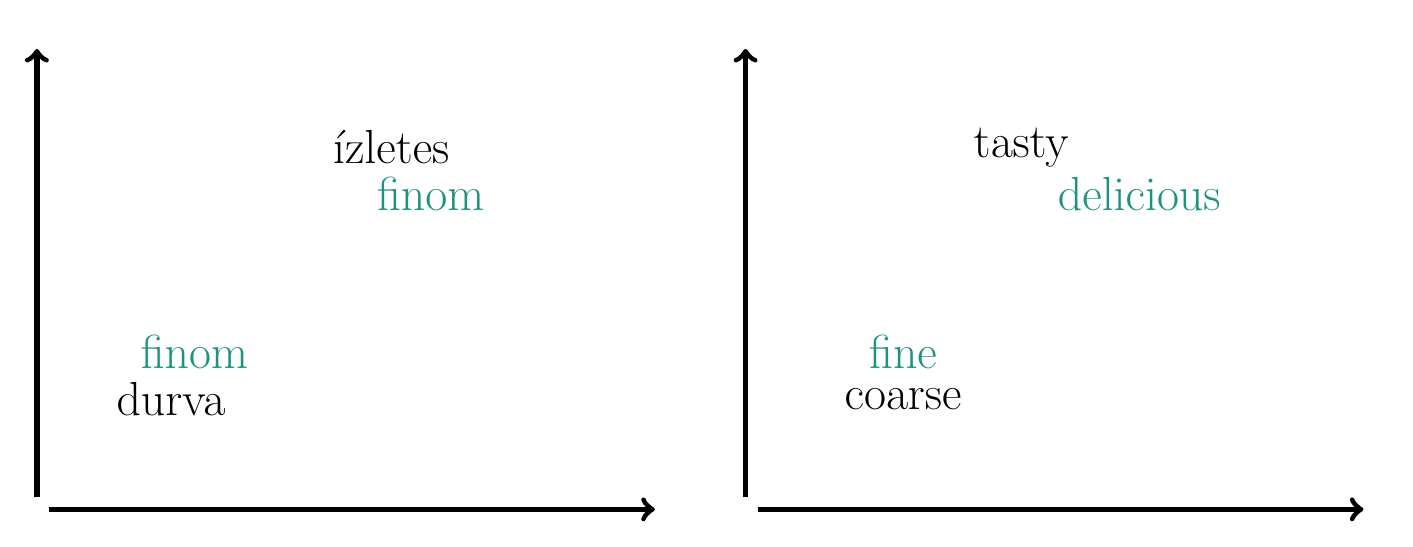
\begin{tikzpicture}[line width=2pt] %[&gt;=stealth']
            \tikzstyle{every node}=[font=\LARGE]
            %\tikzset{every edge thick}
            \node[text=hltdarkgreen] (hf) at (2, 2) {finom};
            \node (hf) at (1.7, 1.4)  {durva};
            \node[text=hltdarkgreen] (hs) at (5, 4)  {finom};
            \node (hs) at (4.5, 4.6)  {ízletes};
            \node[text=hltdarkgreen] (gf) at (11, 2) {fine};
            \node (gf) at (11, 1.4) {coarse};
            \node[text=hltdarkgreen] (gs) at (14, 4) {delicious};
            \node (gs) at (12.5, 4.6) {tasty};
            \node (ho) at (0, 0) {};
            \node (hx) at (8, 0) {};
            \node (hy) at (0, 6) {};
            \node (go) at (9,0) {};
            \node (gx) at (17,0) {};
            \node (gy) at (9,6) {};

            \draw[->] (ho) edge (hx);
            \draw[->] (ho) edge (hy);
            \draw[->] (go) edge (gx);
            \draw[->] (go) edge (gy);
          \end{tikzpicture}
        }
        % \caption{Linear translation of word senses. The Hungarian word
        % \emph{fine} is ambiguous between `fine 'and' delicious'.}
        % \label{fig: AdaGram}
      \end{figure}
\end{frame}

\begin{frame}{Problem: synonymous translations}
  \begin{figure}
    \centering
      \resizebox{\textwidth} {!} {%
        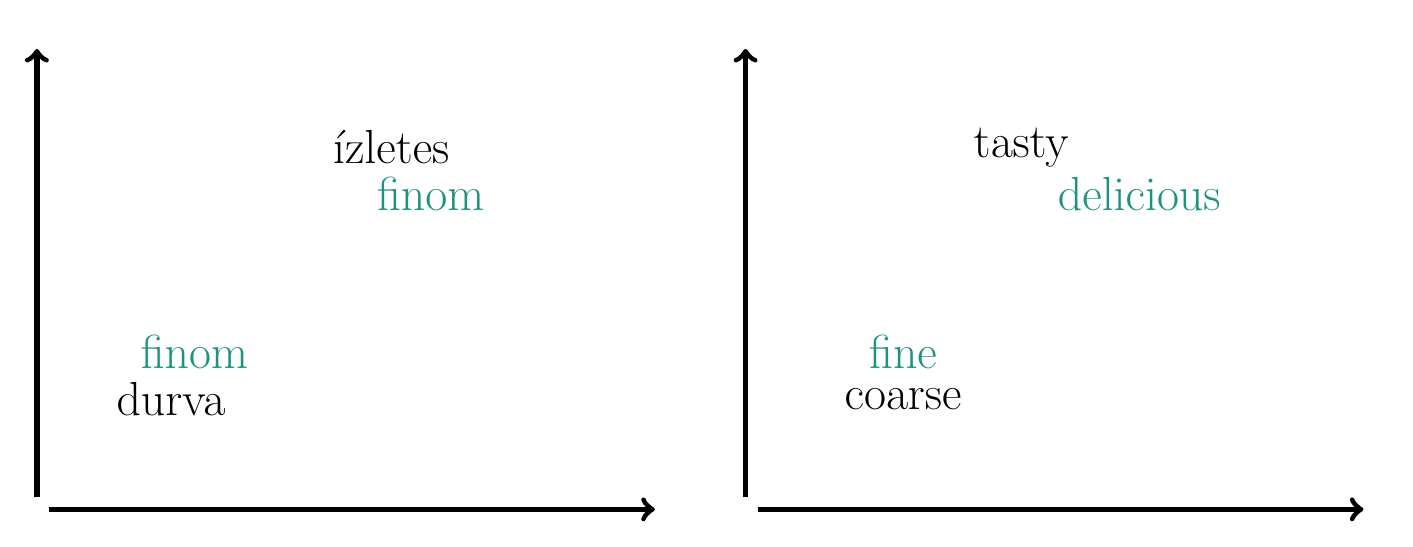
\begin{tikzpicture}[line width=2pt] %[&gt;=stealth']
          \tikzstyle{every node}=[font=\LARGE]
          %\tikzset{every edge thick}
            \node[text=hltdarkgreen] (hf) at (2, 2) {finom};
            \node (hf) at (1.7, 1.4)  {durva};
            \node[text=hltdarkgreen] (hs) at (5, 4)  {finom};
            \node (hs) at (4.5, 4.6)  {ízletes};
            \node[text=hltdarkgreen] (gf) at (11, 2) {fine};
            \node (gf) at (11, 1.4) {coarse};
            \node[text=hltdarkgreen] (gs) at (14, 4) {delicious};
            \node (gs) at (12.5, 4.6) {tasty};
            \node (ho) at (0, 0) {};
            \node (hx) at (8, 0) {};
            \node (hy) at (0, 6) {};
            \node (go) at (9,0) {};
            \node (gx) at (17,0) {};
            \node (gy) at (9,6) {};

            \draw[->] (ho) edge (hx);
            \draw[->] (ho) edge (hy);
            \draw[->] (go) edge (gx);
            \draw[->] (go) edge (gy);
        \end{tikzpicture}
      }
      % \caption{Linear translation of word senses. The Hungarian word
      % \emph{fine} is ambiguous between `fine 'and' delicious'.}
      % \label{fig: AdaGram}
  \end{figure}
\end{frame}
\begin{frame}{Data}
  \begin{itemize}
    \item source corpus
      \bull{
      de-glutinized version \citep{Borbely:2016d,Nemeskey:2017} of the
      Hungarian National Corpus \citep{Oravecz:2014}}
    \item target embedding: GloVe 840B 300d \citep{Pennington:2014}
    \item seed dictionary: wikt2dict \citep{Acs:2013}
    \item training on the first meaning
  \end{itemize}
\end{frame}

\begin{frame}{Evaluation metrics}
    \begin{itemize}
      \item different vectors $ \xRightarrow ? $ different meanings
      \item selection of parameters and target embedding 
        \bull{at least one meaninging vector should have a good translation}
      \item different sense vectors should have a different set of good
        translations 
        \bull{ratio of such items among those predicted to be ambiguous}
    \end{itemize}
  \end{frame}
    \begin{frame}
      \begin{table}[allowframebreaks]
        % \Resizebox {\columnwidth} {!} {%
        \begin{tabular}{lcccc|cc}
          \toprule
          & dim & $\alpha/\gamma$ & $p$ & $m$ & any & disamb \\
          % & \multicolumn{6}{c|}{forward NN search} & \multicolumn{6}{c}{reverse NN search} \\
          %vocab cutoff &&&&& \multicolumn{2}{c}{8192} & \multicolumn{2}{c}{16384} & \multicolumn{2}{c|}{32768} & \multicolumn{2}{c}{8192} & \multicolumn{2}{c}{16384} & \multicolumn{2}{c}{32768} \\
          \midrule
          %/jiweil/mnsz/stemmed/mnsz-stemmed-CRP-800-w15-joint_vect_sense.mse 23.0% 2.200%
          %/jiweil/mnsz/stemmed/mnsz-stemmed-CRP-800-w15-joint_vect_sense_context.mse 26.1% 3.300%
          %/neelakantan/mnsz/stemmed/mnsz2-stemmed-neela-np-800-s2_cluscent.mse 36.3% 6.400%
          %/neelakantan/webkorp_1-sense_sense.mse 37.8% 5.900%
          %/neelakantan/mnsz/stemmed/mnsz2-stemmed-neela-np-800-s2_sense.mse 38.1% 6.500%
          HNC	        & 800	& .02	&       & 100   & 48.5\%	&  7.6\% \\
          \neela~Wk&300&--&2   &big  & 54.0\%	&  12.4\% \\
          HNC stem & 800	& .05	&       &  big & 55.1\%	&  10.4\% \\
          %	& \mutli~Webkorp\footnotemark  &&&&    & 1.0 & 55.0% 13.5\% \\
          HNC         & 160 & .05 & 3     & 200   & 62.2\%	&  15.0\% \\
          \mutli~Wk &300&.25 &       & 71    & 62.9\%	&  17.4\% \\
        Webkorpusz	    & 800	& .05	&       & 100	  & 65.9\%	&  17.4\% \\
        HNC	        & 600	& .05	& 5     & 100	  & 68.6\%	&  16.6\% \\
        HNC	        & 600	& .1  & 3     & 50	  & 69.1\%	&  18.8\% \\
        Webkorpusz	    & 800	& .1  &       & 100	  & 73.9\%	&  23.9\% \\
        \bottomrule
    \end{tabular}
    %}
  \end{table}
\end{frame}

  \begin{frame} [allowframebreaks] {Similarity of good translations}
    \small
    \begin{longtable}{lllll}
      %\setlength{\tabcolsep}{3pt}
      %\resizebox{\textwidth}{!}{%
      %\centering
      \toprule
      %&$s$     &         &                       & covg \\
      %\midrule
        E	& -0.04849	& függő	& addict, aerial	& 0.4 \\
        S	& 0.01821	& alkotó	& constituent, creator	& 0.5 \\
        S	& 0.05096	& előzetes	& preliminary, trailer	& 1.0 \\
        S	& 0.0974	& kapcsolat	& affair, conjunction, linkage	& 0.33 \\
        I	& 0.1361	& kocsi	& coach, carriage	& 1.0 \\
        S	& 0.136	& futó	& runner, bishop	& 1.0 \\
        S	& 0.1518	& keresés	& quest, scan	& 0.67 \\
        S	& 0.1574	& látvány	& outlook, scenery, prospect	& 0.6 \\
        S	& 0.1626	& fogad	& bet, greet	& 1.0 \\
        S	& 0.1873	& induló	& march, candidate	& 1.0 \\
        I	& 0.187	& nemes	& noble, peer	& 0.67 \\
        E	& 0.1934	& eltérés	& variance, departure	& 0.4 \\
        E	& 0.1943	& alkalmazás	& employ, adaptation	& 0.33 \\
        S	& 0.2016	& szünet	& interval, cease, recess	& 0.43 \\
        E	& 0.2032	& kezdeményezés	& initiation, initiative	& 1.0 \\
        S	& 0.2052	& zavar	& disturbance, annoy, disturb, turmoil	& 0.57 \\
        S	& 0.2054	& megelőző	& preceding, preventive	& 0.29 \\
        IE& 0.2169	& csomó	& knot\id, lump\id, mat\e	& 1.0  \\
        E\footnotemark
        & 0.21	& remény	& outlook, promise, expectancy	& 0.6	  \\
        S	& 0.2206	& bemutató	& exhibition, presenter	& 0.67 \\
        E	& 0.2208	& egyeztetés	& reconciliation, correlation	& 0.5 \\
        S	& 0.237	& előadó	& auditorium, lecturer	& 0.67 \\
        E	& 0.2447	& nyilatkozat	& profession, declaration	& 0.4 \\
        I	& 0.2494	& gazda	& farmer, boss	& 0.67 \\
        I	& 0.2506	& kapu	& gate, portal	& 1.0 \\
        I	& 0.2515	& előbbi	& anterior, preceding	& 0.67 \\
        I	& 0.2558	& kötelezettség	& engagement, obligation	& 0.67 \\
        E	& 0.265	& hangulat	& morale, humour	& 0.5 \\
        E	& 0.2733	& követ	& succeed, haunt	& 0.67 \\
        SE	& 0.276	& minta	& norm\s, formula\e, specimen\s	& 0.75  \\
        S	& 0.2807	& sorozat	& suite, serial, succession	& 1.0 \\
        S	& 0.2935	& durva	& coarse, gross	& 0.18 \\
        I	& 0.3038	& köt	& bind, tie	& 0.67 \\
        E	& 0.3045	& egyezmény	& treaty, protocol	& 0.67 \\
        I	& 0.3097	& megkülönböztetés	& discrimination, differentiation	& 0.5 \\
        I	& 0.309	& ered	& stem, originate	& 0.5 \\
        I	& 0.319	& hirdet	& advertise, proclaim	& 1.0 \\
        E	& 0.3212	& tartós	& substantial, durable	& 1.0 \\
        I	& 0.3218	& ajánlattevő	& bidder, supplier, contractor	& 0.6 \\
        I	& 0.3299	& aláírás	& signing, signature	& 0.67 \\
        I	& 0.333	& bír	& bear, possess	& 1.0 \\
        I	& 0.3432	& áldozat	& sacrifice, victim, casualty	& 1.0 \\
        IE	& 0.3486	& kerület	& ward\id, borough\id, perimeter\e	& 0.3  \\
        I	& 0.3486	& utas	& fare, passenger	& 1.0 \\
        I	& 0.3564	& szigorú	& stern, strict	& 0.5 \\
        I	& 0.3589	& bűnös	& sinful, guilty	& 0.5 \\
        I	& 0.3708	& rendes	& orderly, ordinary	& 0.5 \\
        I	& 0.3824	& eladó	& salesman, vendor	& 0.5 \\
        I	& 0.3861	& enyhe	& tender, mild, slight	& 0.6 \\
        I	& 0.3897	& maradék	& residue, remainder	& 0.33 \\
        I	& 0.3986	& darab	& chunk, fragment	& 0.4 \\
        E	& 0.4012	& hiány	& poverty, shortage	& 0.5 \\
        %I	& 0.4093	& kutatás	& exploration, quest	& 0.5 \\
        %I	& 0.4138	& tanítás	& tuition, lesson	& 0.67 \\
        %I	& 0.4196	& őszinte	& frank, sincere	& 0.67 \\
        %I	& 0.4229	& környék	& neighborhood, surroundings, vicinity	& 0.38 \\
        %I	& 0.4446	& ítélet	& judgement, sentence	& 0.67 \\
        %I	& 0.4501	& gyerek	& childish, kid	& 0.67 \\
        %I	& 0.4521	& csatorna	& ditch, sewer	& 0.4 \\
        %I	& 0.4547	& felügyelet	& surveillance, inspection, supervision	& 0.43 \\
        %E	& 0.4551	& ritka	& rare, odd	& 0.5 \\
        %S	& 0.4563	& szerető	& fond, lover, affectionate, mistress	& 0.67 \\
        %I	& 0.4608	& szeretet	& affection, liking	& 0.67 \\
        %I	& 0.4723	& vizsgálat	& inquiry, examination	& 0.67 \\
        %I	& 0.4853	& tömeg	& mob, crowd	& 0.5 \\
        %I	& 0.4903	& puszta	& pure, plain	& 0.22 \\
        %I	& 0.4904	& srác	& kid, lad	& 1.0 \\
        %I	& 0.4911	& büntetés	& penalty, sentence	& 0.29 \\
        %I	& 0.4971	& képviselő	& delegate, representative	& 0.67 \\
        %I	& 0.4975	& határ	& boundary, border	& 0.67 \\
        %I	& 0.5001	& drága	& precious, dear, expensive	& 1.0 \\
        %S	& 0.5093	& uralkodó	& prince, ruler, sovereign	& 0.5 \\
        %I	& 0.5097	& válás	& separation, divorce	& 0.67 \\
        %I	& 0.5103	& ügyvéd	& lawyer, advocate	& 0.67 \\
        %I	& 0.5167	& előnyös	& advantageous, profitable, favourable	& 1.0 \\
        %I	& 0.5169	& merev	& rigid, strict	& 1.0 \\
        %I	& 0.5204	& nyíltan	& openly, outright	& 1.0 \\
        %I	& 0.5217	& noha	& notwithstanding, albeit	& 1.0 \\
        %I	& 0.5311	& hulladék	& litter, garbage, rubbish	& 0.43 \\
        %I	& 0.5311	& szemét	& litter, garbage, rubbish	& 0.43 \\
        %I	& 0.5612	& kielégítő	& satisfying, satisfactory	& 1.0 \\
        %E	& 0.5617	& vicc	& joke, humour	& 1.0 \\
        %I	& 0.5737	& szállító	& supplier, vendor	& 1.0 \\
        %I	& 0.5747	& óvoda	& nursery, daycare, kindergarten	& 1.0 \\
        %I	& 0.5754	& hétköznapi	& mundane, everyday, ordinary	& 0.75 \\
        %I	& 0.5797	& anya	& mum, mummy	& 1.0 \\
        %I	& 0.5824	& szomszédos	& neighbouring, neighbour	& 0.4 \\
        %E	& 0.5931	& szabadság	& liberty, independence	& 1.0 \\
        %I	& 0.6086	& lelkész	& pastor, priest	& 0.4 \\
        %I	& 0.6304	& fogalom	& notion, conception	& 1.0 \\
        %I	& 0.6474	& fizetés	& salary, wage	& 0.67 \\
        %I	& 0.6551	& táj	& landscape, scenery	& 1.0 \\
        %I	& 0.6583	& okos	& clever, smart	& 0.67 \\
        %I	& 0.6707	& autópálya	& highway, motorway	& 0.5 \\
        %I	& 0.6722	& tilos	& prohibited, forbidden	& 1.0 \\
        %I	& 0.6811	& bevezető	& introduction, introductory	& 1.0 \\
        %I	& 0.7025	& szövetség	& coalition, alliance, union	& 0.75 \\
        %I	& 0.7065	& fáradt	& exhausted, tired, weary	& 1.0 \\
        %I	& 0.7066	& kiállítás	& exhibit, exhibition	& 0.67 \\
        %I	& 0.7135	& hirdetés	& advert, advertisement	& 1.0 \\
        %I	& 0.7147	& ésszerű	& rational, logical	& 1.0 \\
        %I	& 0.7664	& logikai	& logic, logical	& 1.0 \\
        %I	& 0.7757	& szervez	& organise, organize, arrange	& 1.0 \\
        %I	& 0.8122	& furcsa	& strange, odd	& 0.4 \\
        %I	& 0.8277	& azután	& afterwards, afterward	& 0.67 \\
        %I	& 0.8689	& megbízható	& dependable, reliable	& 0.67 \\
    \bottomrule
    %}
    % \caption{Hungarian words with the rNN@1 translations of their sense
    % vectors.  The first column is a post-hoc annotation by András Kornai
    % (\emph E error in translation, \emph I identical, \emph S separate
    % meanings), $s$ is the cosine similarity of the translations, and
    % \emph{covg} denotes the coverage of the @1 translations over all gold
    % translations.}
  \end{longtable}
  %\label{tab:alkoto}
  %{\footnotesize $^7$ The basic translations \emph{hope} is missing}
\end{frame}
%\begin{frame} { Conclusion}
%  \begin{itemize}
%    \item input: corpus in two languages + 5 thousand translation pairs
%    \item resource: disambiguated translation of the corpus vocabulary
%    \item research result: separating the types of polysemy
%      cosine (we've verified words that are the same
%      translations)
%    \item move: the various multiplayer skip-gram models
%      more systematic examination
%  \end{itemize}
%\end{frame}
%\begin{frame} {Main Performer's Publications}
%  \newcommand{\vspacelast}{\vspace{6mm}}
%  \vspacelast
%  \centering \url{https://github.com/makrai/wsi-fest}
%  \vspacelast
%  \begin{itemize}
%    \item A \fl~conceptual dictionary \\ \citep{Kornai:2013,Kornai:2015a}
%      \begin{itemize}
%        \item igei roles \citep{Makrai:2014}
%        \item is the defining vocabulary \citep{Makrai:2013a,Kornai:2015a}
%        \item activation projection \citep{Nemeskey:2013}
%      \end{itemize}
%    \item wordings
%      \begin{itemize}
%        \item\alert{lexical relations} \citep{Makrai:2013b,Makrai:2014b}
%        \item for European languages \citep{Makrai:2015,Makrai:2015b}% MSZNY, CogInfoCom
%        \item vectors in the brain \citep{Makrai:2014p}
%        \item ambiguity triangulation \citep{Makrai:2016l}
%        \item multi-report embedding (MSEk) \\ (\cite{Borbely:2016},Makrai (under review))
%      \end{itemize}
%  \end{itemize}
%\end{frame}
\begin{frame} [allowframebreaks] {Bibliography}
  \printbibliography
\end{frame}

\begin{frame} [allowframebreaks] {Tricks for Linear Translation}
  \begin{itemize}
    \item inverse neighbors
      \begin{itemize}
        \item hubs for NN search \citep{Radovanovic:2010}
        \item inverted neighbors \citep{Singh:2003}
        \item for linear translation \citep{Dinu:2015,Lazaridou:2015}
      \end{itemize}
    \item orthogonal constraint
      \begin{itemize}
        \item originally has three types of spacing
          \begin{itemize}
            \item is a scalar for embedding training
            \item when training the mapping Euclidean
            \item translation
          \end{itemize}
        \item unification \citep{Xing:2015,Faruqui:2014,Artetxe:2016}
          \begin{itemize}
            \item vectors are normalized
            \item orthogonal mapping: rotates but does not provide
            \item centering?
          \end{itemize}
      \end{itemize}
  \end{itemize}
\end{frame}
\end{document}
